\chapter{Use Case Implementation}

The project includes a demonstration of Use Case 1 from Chapter \ref{chapter:use_case_1}. The implementation has been done on several ESP32 board running FreeRTOS which are both described in Chapter \ref{chap:freertos}. The keylogger application is built and deployed on one of the ESP's dual cores. The other one is used to fulfill the specifications of the use case. \\

The keylogger application was built using the ESP-IDF with resources from the FreeRTOS documentation and the ESP-IDF example projects, as well as other projects that can be found online. All the code that is discussed in this segment can be found in the project's \href{https://github.com/C4ES-PoliTO/FreeRTOS-Monitoring}{\textbf{github repository}}.

\section{ESP-IDF}
This project deploys as previously mentioned FreeRTOS on an ESP32 board \cite{manual:ESP-IDF}. The Espressif IoT Development Framework is a development environment containing build tools and \hyperlink{https://github.com/espressif/esp-idf/tree/master/examples}{\textbf{example projects}} as extensions for the Visual Studio Code and Eclipse IDEs. 

These resources can be used on top of the minimal version of FreeRTOS to support several communication protocols, tracing and other functionalities useful for a keylogger.

\section{Network topology}
As is described in the Use Case 1, we are dealing with a set of patients carrying the monitoring devices, they form a star topology together with a gateway, which can be either carried by a nurse or fixed in a given location. In order to achieve a robust connection and to facilitate the collection of network parameters and traffic, we have set up the central node to work as an Access Point and create a Wi-fi network which the patients connect to. More information on monitoring the network traffic will be provided in the section \ref{sec:CentralNodeMonitoring}

\begin{figure}[h]
    \centering
    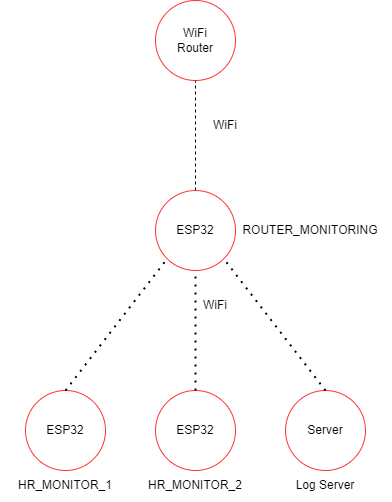
\includegraphics[scale=0.5]{images/uc_topology.png}
    \caption{Network topology of use case 1.}
    \label{fig:uc1}
\end{figure}


\section{Monitoring the devices}
Firstly, we have undergone a process of transforming the user requirements (Use case specifications) into technical objectives set for development. When studying the architecture of the ESP32 in this solution, we can see that it offers a very attractive feature in terms of monitoring capabilities: A dual core.\\ 

This dual core enables a user application to be deployed in the first core (Core 0), supported by FreeRTOS. The \textbf{monitoring tasks} deployed on the second core (Core 1) focus on "spying" on the application to collect different kinds of data and extract vital information from it. One example of this is our monitoring task can check what sockets are being used at any given time, collect the IPs and examine whether the device is communicating with an unexpected source.
\\~\\
Now we will cover the implementation of the different monitoring techniques that have been applied to both the leaf nodes and the central node in our IoT solution.


\subsection{Code Structure}
As a preface, it is important to remark that the code is divided in two main segments, contained in the "Source\_code" folder of the github repository. The first contains all aspects of the leaf node. The (esp32\_leaf\_node) folder is built and flashed onto the ESP32 that act as the leaf nodes.
\\~\\
The second segment is the one contained in the folder "esp32\_nat\_router", this one is built and flashed onto the esp32 which acts as the central router.
\\~\\
Another approach would have been to merge the codes and have some kind of variable similar to IS\_LEAF\_NODE which determined the program flow to follow, but due to development, readability and reusability concerns we have decided to separate and modularize the code in this form.


\subsection{Leaf node monitoring}
In this use case, the leaf nodes measure vital information from the patients, then sends it to the gateway to be transferred to a server which makes sure all the patients are at good health.
\\~\\
However, we have aimed to abstract the use case and offer a monitoring solution that can be easily implemented in any other use case and still provide valuable information.
\\~\\
When designing the monitoring functions for the leaf node, there are several interesting parameters than can give us important information about how the system is behaving. When researching attacks it was discovered that launching a large number of tasks to be scheduled can become overwhelming for the operative system. This can produce a denial of service attack, especially if the attacker finds a way to launch high-priority tasks that can starve lower priority functionality. The possibility of launching low-priority task to starve high-priority ones could have produced more severe results. However, this is avoided by the priority inheritance feature that is implemented in the operative system in order to avoid priority inversion. \\

Therefore, it was natural to implement a functionality that monitors the number of tasks created within a time interval and use this data to decide whether this could be a potential attack or not. The implementation is based on example code from the ESP-IDF and FreeRTOS API guides \cite{uxTaskGetSystemState} where the vTaskGetRunTimeStats function is used to retrieve real time information about the tasks running on the CPU at a specific moment in time. The information extracted represents the task handle, task name, task priority, task state, and total amount of run time consumed by the task. By probing this at different points in time one can list which tasks have been created or deleted during the last interval in time. \\

All of this information can be sent to the server. Another possibility, which is the intelligent part of the monitoring, is to check the number of created tasks up against some predetermined threshold. It would be the maximum number of tasks to be expected during normal operation. If a node is experiencing an increase in tasks higher than the threshold it sends a message containing the number of created tasks, the number of expected tasks and a list of all the tasks that has been created along with their priorities to also detect potential starvation.\\

\begin{lstlisting}[
  breaklines,
  rulecolor=\color{black},
  frame=single,
  language=C,
  basicstyle=\ttfamily\small
]
void DoS_Monitoring(TaskStatus_t *pxTaskStatusArray, UBaseType_t array_size, int buffer_length, char *writeBuffer, int count) {
    buffer_length += snprintf( writeBuffer + buffer_length, TASK_BUFFER_SIZE - buffer_length,"| DoS suspected, number of created tasks: %u\n", count);
    buffer_length += snprintf( writeBuffer + buffer_length, TASK_BUFFER_SIZE - buffer_length,"| Maximum number of task expected for period: %u\n", THRESHOLD);
    buffer_length += snprintf( writeBuffer + buffer_length, TASK_BUFFER_SIZE - buffer_length,"| Task name | Task base priority \n");
    
    ESP_LOGI(TAG,"DoS suspected, number of created tasks: %d, threshold: %d", count, THRESHOLD);
    
    for (int i = 0; i < array_size; i++) {
        if (pxTaskStatusArray[i].xHandle != NULL) {
            buffer_length += snprintf( writeBuffer + buffer_length, TASK_BUFFER_SIZE - buffer_length,"| %s | %u \n", 
                                    pxTaskStatusArray[i].pcTaskName, 
                                    pxTaskStatusArray[i].uxBasePriority);
        }
    }
}
\end{lstlisting}



This would of course require some knowledge about the application and the normal amount of coexisting tasks. Therefore there are two versions on this monitor - one that outputs all running tasks with belonging information at each time interval, and one that only notifies the network if abnormal amounts of tasks are created.\\

To test the functionality a simple function is run as a part of the testing. This function creates a number of tasks that exceeds the threshold. This triggers the monitor to notify the network. \\


\begin{lstlisting}[
  breaklines,
  rulecolor=\color{black},
  frame=single,
  language=C,
  basicstyle=\ttfamily\small
]
void DoSTask(void * param) {
    int *num1 = param;
    int num = num1;

    while(1) {
        vTaskDelay(pdMS_TO_TICKS(5600));
    }
}

void DoSTest(void) {

    ESP_LOGI(TAG,"DoS test initiated.");

    for(int i = 0; i < THRESHOLD +1; i++) {
        int y = i;
        xTaskCreatePinnedToCore(DoSTask, "DoS test", 4096, y, 3, NULL, 0);
        vTaskDelay(pdMS_TO_TICKS(500));
    }
}
\end{lstlisting}

This monitoring functionality is also added to the central node. The only adaptation that needs to be made is altering the threshold to match the expected number of tasks for this type of node.

The CPU usage of a task can be included to see if the task is receiving inputs that leads it to use abnormal amounts of capacity. This is on the other hand very application dependent, but it could in future implementation check for abnormal portions of capacity. 

\subsection{Socket monitoring}
As part of the leaf monitoring, it is really important to log the network traffic at the device. Specifically, logging the metadata is fundamental, as it provides the destination IP/port, and the size of the message. Since this use case considers a deterministic scenario, all network destinations and sources, as well as the data size range are known in advance. If the log does not match the whitelisted IPs, it is easy to recognize that data is being leaked. In the same way, if the size of the message is much bigger than expected, it could mean that a DoS attack is in process.\\

In order to be able to log all network traffic, independently from the application level, we must resort to the device's sockets. ESP-IDF's network stack relies on the LWIP library, therefore, by modifying the lwip/sockets.c functions it is possible to access to this information, both for UDP and TCP packets.\\

The following functions have been duplicated and modified to log and send the message's metadata to a remote server where it can be analyzed. 
\begin{itemize}
    \item lwip\_recvfrom()
    \item lwip\_send()
    \item lwip\_sendto()
\end{itemize}
Since we do not want to monitor the messages sent by this monitoring task, as it would create an infinite loop, the original functions are also kept, but with a different name, and used only by the monitoring task. Here is an example of the added functionality to the lwip\_send() function. The data is extracted by the corresponding structures, and then sent to UDP server by the created udp\_send\_msg(). 
\begin{lstlisting}[
  breaklines,
  rulecolor=\color{black},
  frame=single,
  language=C,
  basicstyle=\ttfamily\small
]
    ip_addr_t addr;
    u16_t port;
    netconn_peer(sock->conn, &addr, &port);
    char msg_data[1024];
    sprintf(msg_data, "(%s) TCP connection to Socket: %d, IP: %s, Port 
    udp_send_msg(UDP_SERVER_IP, UDP_SERVER_PORT, msg_data);
\end{lstlisting}


\subsection{Central node monitoring} \label{sec:CentralNodeMonitoring}
Another "level" which offers very valuable information is the network, in this regard, we have designed some monitoring tasks that, while not completely application independent, offer a high degree of reusability and portability into other solutions similar to ours.
\\~\\
To fully leverage all the network monitoring capabilities, we have decided for our central node to act as an \textbf{access point} to the rest of nodes, which will connect to it. The node will be then in charge or relaying the information to an external server, in essence acting as a more "intelligent" router. To aid in the implementation of this code, which is not the objective of this project, we have used some code present in \href{https://github.com/martin-ger/esp32_nat_router}{\textbf{this github repository}}, while other resources have been learned through the study of several examples present in \href{https://github.com/espressif/esp-idf/tree/master/examples}{\textbf{Espressif's example projects}}, mainly "SoftAP".
\\~\\
Since we are aiming for an abstraction from the application level, we will not consider the content of the messages or their recipients, though this would also be valid information (And they are partially covered by socket monitoring in the leaf nodes), in fact we will not consider the messages at all, the only parameters we will consider are:

\begin{itemize}
    \item Number of connected stations
    \item MAC addresses of stations
\end{itemize}


Let us analyze these parameters and why they might be interesting from a security point of view. In most use cases related to the one we have based ourselves upon, the number of connected nodes will be relatively stable throughout defined periods of time, therefore if any anomalies in the number of connected nodes is detected, it is very important to relay this to an external server. A bigger than expected number of nodes can indicate that malicious nodes are present in our system, with the ensuing risk, on the other hand, a number of connected nodes smaller than the expected might mean that we have suffered a DoS attack on a number of them, or that our central node has been compromised.\\~\\

The other parameter we are monitoring is the MAC address of our connected devices, the monitoring task has a list of whitelisted MAC addresses, if a MAC address not in this list connects to the wifi, an alarm is sent to the server.\\~\\

The script in charge of monitoring these parameters is \textbf{router\_monitoring.c}, located inside the "main" folder of "esp32\_nat\_router". A FreeRTOS task is created in the main code, linking this task to Core 1. The task first defines an event handler for the event type \href{https://docs.espressif.com/projects/esp-idf/en/latest/esp32/api-reference/system/esp_event.html}{\textbf{system\_event\_base\_t}} which can bee seen in Figure \ref{fig:wifi_event_handler}. 

\begin{figure}[H]
\centering
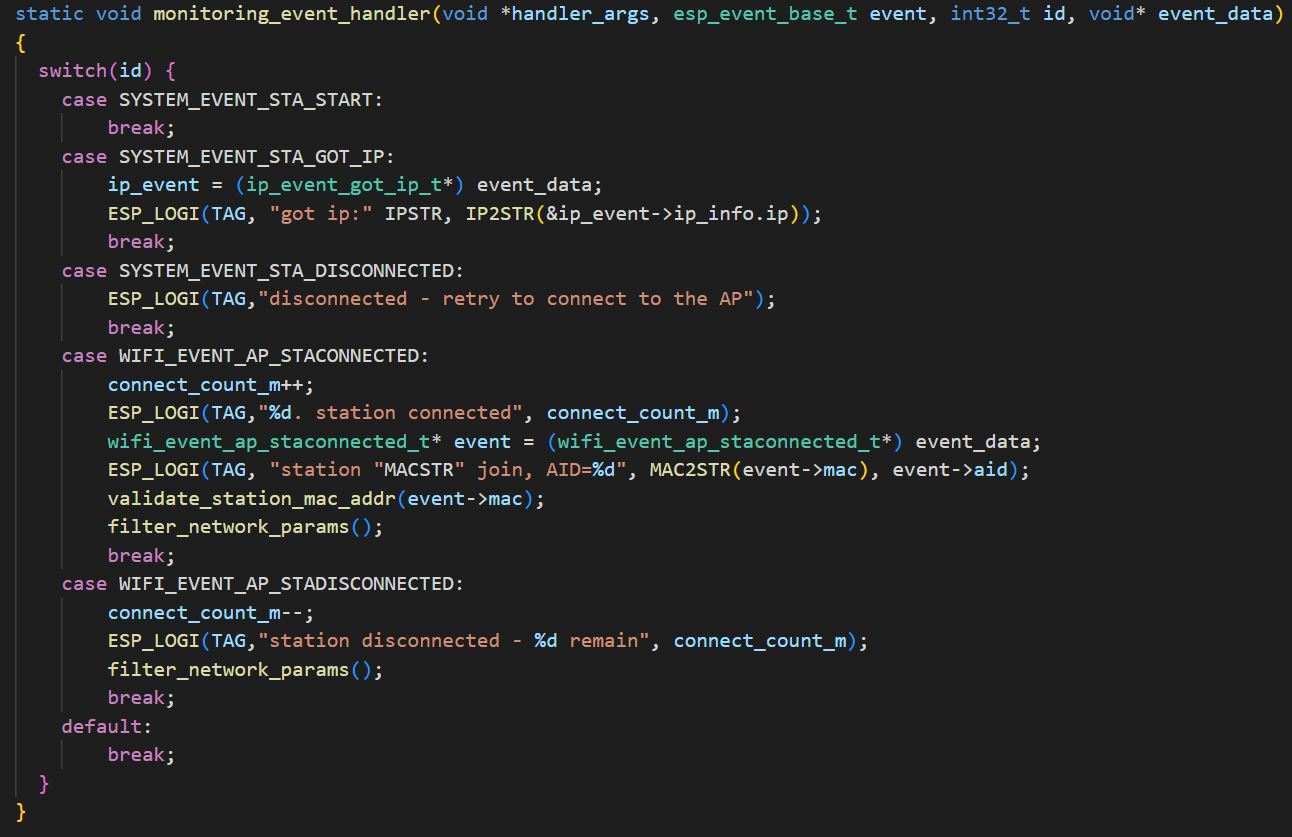
\includegraphics[width=.9\linewidth]{images/wifi_event_handler_code.JPG}
\caption{Wifi event handler code in routerMonitorin.c}
\label{fig:wifi_event_handler}
\end{figure}

This handler is then posted to the \href{https://docs.espressif.com/projects/esp-idf/en/latest/esp32/api-reference/system/esp_event.html}{\textbf{default system event loop}}, which allows the event handler to handle the incoming events, the events we will react to are:

\begin{itemize}
    \item \textbf{WIFI\_EVENT\_AP\_STACONNECTED: } This event is posted to the event loop when a station connects to our Access Point, our monitoring task then checks that its MAC address is whitelisted, if it is not an alarm is raised to the server. The handler also calls \textbf{filter\_network\_params()}, which keeps track of the number of connected stations and checks that it is whithin an expected range, if this is not met an alarm is sent to the server.
    
    \item \textbf{WIFI\_EVENT\_AP\_STADISCONNECTED: } This event is posted to the event loop when a station disconnects, the handler then calls \textbf{filter\_network\_params()} to check that the number of connected stations is in an expected range.
    
\end{itemize}

If any anomalies described above are detected, the monitoring task opens a udp socket to communicate with the monitoring server which receives the alerts.

\begin{figure}[H]
\centering
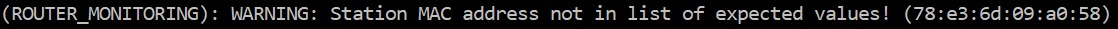
\includegraphics[width=.9\linewidth]{images/monitoring_warning_mac_whitelist.jpeg}
\caption{Alert message recieved by the server when an unexpected MAC addr connects}
\label{fig:monitoring_alert_mac}
\end{figure}

\begin{figure}[H]
\centering
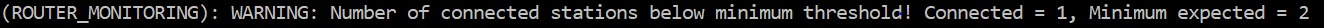
\includegraphics[width=.9\linewidth]{images/monitoring_warning_minimum_stations.jpeg}
\caption{Alert message recieved by the server when too few stations are connected}
\label{fig:monitoring_alert_few_stas}
\end{figure}

\begin{figure}[H]
\centering
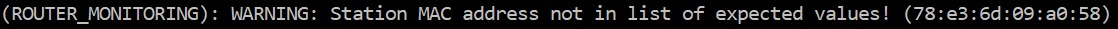
\includegraphics[width=.9\linewidth]{images/monitoring_warning_mac_whitelist.jpeg}
\caption{Alert message recieved by the server when too many stations are connected}
\label{fig:monitoring_alert_many_stas}
\end{figure}